\chapter{Frontends}
\label{chapter:frontend}

\chapterprecishere{As far as the laws of mathematics refer to reality, they are not certain; and as far as they are certain they do not refer to reality.\par\raggedleft--- \textup{Albert Einstein}}
\chapterhung

\index{frontend|boldindex}

A reusable way to provide functionality to different applications is via \empha[application programming interface (API)]{APIs}.
API design is known to be important and challenging~\cite{block2006api,grill2012methods,thomas2006api,burns2016borg,russell2008virtio}.
For developers, ideally the visible part of configuration access is reduced to an API.
In this chapter, after a short discourse of the history of \elektra{}'s APIs, we present three high-level, type-safe, and context-aware APIs.
Furthermore, we elaborate on design choices, discuss extensions, find rationales for requirements, and tackle the research question:
\rqFrontend*

\section{History of \textsc{Elektra}'s APIs}
\label{sec:api-history}

Here we describe earlier versions of \elektra{}'s APIs and strive to answer \rqref{frontend-design-decisions}:
\rqFrontendDesignDecisions*

Similar to programming languages~\cite{landin1966next} and data description languages~\cite{fisher2010next} the design space for configuration access is vast.
Here we discuss design choices of \elektra{}'s API and observations that lead us to the high-level APIs presented in this chapter.




Let us start with API functionality that survived unchanged for 13 years (2004--2017):

\begin{enumerate}
\item
It is useful to pass to the user only data structures exclusively accessible via API.
Among many advantages, the data structure allows internal reorganizations and optimizations without changes visible to the user.
\begin{example}
The configuration access API ^getenv^ that does not prohibit direct access to ^environ^ is a negative example.
Because of direct access to ^environ^, ^getenv^ invocations give neither guarantees with respect to thread-safety nor about availability of the pointer passed back.
Furthermore, ^environ^ is easily tricked into having duplicated entries.
\end{example}


\item
\elektra{}'s data structure is a set composed of individual records (and not only strings) throughout the whole API's lifetime.
Doing so had many advantages for advanced lookup strategies and for providing metadata.

\item
It is a good idea to fully take control over memory management and always provide pairs of functions for opening and closing resources.
Even though the details changed completely, all attempts to do otherwise failed completely.
The abstraction proved to be useful, for example, when introducing an ^mmap^ cache.

\item
\elektra{} always emitted a data structure and never was event-driven~\cite{laemmel2011ast}.
Since later versions, hooks for updates on changes have been possible via plugins.
With \elektra{}, applications do not have to implement their own data structure for configuration settings.
Other reasons for the data structure are its need for plugins, conversions, and frontends.
\end{enumerate}


\subsection{Abstraction}

The first API of \elektra{} offered operations that supported modifications of both persisted single keys and persisted key sets.
From an implementation point of view this duality complicated the implementation of backends:
Backends needed to implement both ways.
It is, however, difficult to partially serialize configuration files, as it would be needed for setting a single key.
We decided to put a focus on supporting configuration files by only supporting key set (and not key) operations in the backend.
Modifications of single keys were moved to convenience APIs.

In \elektra{}~0.6 released on \formatdate{30}{3}{2006}, \elektra{} described changes that shall be applied to the current configuration settings.
For example, the API user had to explicitly remove keys if they were no longer wanted.
This behavior was problematic for configuration files.

In \elektra{}~0.7 released on \formatdate{17}{10}{2008}, we used a hybrid approach~\cite{raab2010thesis}:
In a key set we described the complete configuration settings as they shall be applied.
Furthermore, we described the differences of which keys were removed since parsing the configuration files.
This was an efficient method for configuration files as well as other backends.
Unfortunately, the API was not intuitive:
To remove a key, one needed to mark the key for removal instead of removing it from the key set.
When simply removing keys from the key set, it would not necessarily be removed in the backend.
Furthermore, this API required us to sort keys in the ^KeySet^ specially:
The keys marked for removal had to be separated from the other keys.

Since \elektra{}~0.8.0~\cite{raab2010thesis} implemented in 2010, released on \formatdate{5}{5}{2012}, we fully migrated to a system, where the key set contains the complete configuration settings.
The correlation of in-memory key set and configuration files  is an instance of the view-update problem~\cite{foster2010bidirectional}.
The state represents a view of the configuration files.
Changes in the state must be translated back to configuration files.

\paragraph{API evolution:}
To mitigate many problems of API evolution a proposal process proved to be  helpful.
Instead of directly adding to the API, developers first need to propose their change.
This change is only accepted in a library that is specifically marked to contain proposed enhancements.
When the demand is clearly given and no further improvements to the API are suggested, the API is moved to the core.
\newcommand{\supportedbindings}{C++, Python, Haskell, Lua, Shell, Ruby, and Java}
The API stagnated and stayed minimal, which eased the development of the bindings for \supportedbindings; and we fulfilled the requirement:
\reqMinimal*


\subsection{Context}
\label{sec:frontend-history-context}

Already before starting with the dissertation we had the intuition that key-value-based configuration access APIs alone had limitations in combination with some requirements.
We wanted to implement a software stack for an embedded computer with a connected camera.
The cameras needed various non-trivial configuration settings in order to work, for example, shutter speed and sensor sensitivity.

The challenging part was to easily switch connected cameras and add new cameras without changing the source code.
Every camera needed different configuration settings but also had substantial overlap with configuration settings of other cameras.

The na\"{\i}ve object-oriented way is to implement the configuration procedure of every camera as subclass of a camera class.
The configuration settings are for the camera objects to be instantiated.
This solution fails in the requirement of the ability to add new cameras without source code changes.
Furthermore, these classes would hardly describe any behavior;
They mostly describe different values for different cameras, which is not the strength of object-oriented programming.

In an abstract viewpoint the connected camera is part of the configuration setting.
But from the viewpoint of the application it is not configuration settings:
It is something given from the outside world.
We have to adapt our configuration settings to the constraints we have from the environment.
We did not find an elegant solution within object-oriented programming for such constraints from the environment.

We came up with a solution by introducing an extension of \empha[profile]{profiles}.
In our extension, developers specify several profiles:
If a configuration setting is not found in the first profile, the search continues in the second profile, and so on.
So instead of looking up configuration values directly, profiles determine which value we shall use.
In retrospect this feature has been a cascading lookup with manually specified namespaces.
For example, if we use ^ksLookup("shutter_speed", {"model","manufacturer"})^ we look up the shutter speed:
\begin{enumerate}
\item accounting for the profile ^model^, and
\item if the ^shutter_speed^ was not found, we use the ^manufacturer^ profile as fallback.
\end{enumerate}

The API for profiles created a usability problem for developers because:
\begin{itemize}
\item Developers were directly confronted with this concept when using the API.
\item One always had to remember to pass the list of profiles to the correct places.
\item The combination of different profiles was hard to understand due to its flexibility.
\item It inherently has the limitation that profiles are exclusively clustered in a single dimension.
\end{itemize}

Some time after the camera project, we found context-oriented programming to be a perfect fit.
Instead of writing a list of profiles in every configuration access point, we write contextual specifications.
The developers specify all dependences towards context in one place.
Instead of the error-prone combination of profiles, we would activate layers.
The environment would be modeled by layers as context-oriented programming proposes.
In this chapter we discuss this idea in detail.


\subsection{Decisions}

\tabref{api-decision} gives a summary of various decisions in \elektra{} and shows which of them were reverted in the current version.

\begin{table}[htp]
\noindent
\begin{tabularx}{\columnwidth}{l  R  R}
\toprule
\multicolumn{1}{l}{\bfseries Decision} &
\multicolumn{1}{R}{\bfseries Earlier versions ($< 0.8$)} &
\multicolumn{1}{R}{\bfseries Current version ($\geq 0.8$)}
\\
\hline
data structure              & list         & custom \\
opaqueness                  & partly       & fully \\
linear search               & yes          & no \\
metadata                    & fixed number & arbitrary \\
memory                      & open\&close  & ref-counted \\
hooks on access             & no           & via plugins \\
XML streaming               & built-in     & via plugins \\
process for API changes     & no           & yes \\
high-level API              & in core      & separated \\
focus in support of storages& no focus     & configuration files \\
sorting                     & manual       & always (at insert) \\
context-aware lookups       & no           & via plugins  \\
configuration specification & informally   & yes         \\
object-oriented API         & yes          & yes         \\
code-generated API          & no           & yes         \\
context-oriented API        & no           & yes         \\
\bottomrule
\end{tabularx}
\caption[Decisions for an API.]{Decisions for an API. The version 0.8.0 was released on \formatdate{5}{5}{2012}.}
\label{tab:api-decision}
\end{table}




























\section{Execution Environment as Contextual Values}
\label{sec:cop}

We suggest facilitating \empha[execution environment]{execution environments} as \empha[contextual value]{contextual values}.
For example, let us employ external configuration settings via ^getenv^ to query the execution environment.
We need to be careful:
After dynamic reconfiguration the settings valid in the new context differ from those obtained with ^getenv^~\cite{raab2014program}.

Next to external context changes, we face another problem:
In some parts of the program the context is more specific than in other parts of the program.
For example, a Web browser has opened private and history-aware tabs at the same time.
Although we want to run the same source code for all tabs, the differences are  important for the user.
To reduce the danger of applying wrong context information it is desirable to ensure that access to execution environments always considers context~\cite{raab2014program}.

Contextual values allow us to safely interact with an execution environment.
They ensure that the context is taken into account when accessing the execution environment~\cite{raab2016persistent}.

We propose to specify the contextual values connected with the execution environment as part of a separate unit.
The separate unit is the configuration specification and consists of external configuration files containing specifications for contextual values.
Such specifications facilitate context placeholders, each representing a dimension of the context awareness of the contextual value~\cite{raab2014program}.

\begin{example}
\label{ex:greeting}
To greet in different languages, we would specify a contextual value:

\begin{code}
[%language%/person/greeting]
  type:=string
  description:=hello in all languages
  default:=Hi!
\end{code}

The basename of the key name (^greeting^) is the name of a contextual value of the type ^string^; and ^%language%^ is a context placeholder to be substituted in contextual interpretations.
\elektra{Gen} yields the contextual class ^Greeting^ using the contextual value specification above~\cite{raab2014program}.
\end{example}

For contextual interpretations, we substitute these context placeholders with values given by layers.
The resulting key name is used with ^ksLookup^.
In addition to the specification, we have a configuration file containing the greetings in different languages:

\begin{code}[language=CfgElektra]
german/person/greeting=Hallo!
\end{code}

In the example above, the contextual value provides two different values with ^%^ for an empty layer.

\subsection{How to use Context Information?}

To work with \elektra{}, developers need to specify the contextual values and layers.
Then developers can immediately facilitate the contextual values in their source code in the same way as variables are used~\cite{raab2014program}.

\begin{example}
\label{ex:contextual-value-greeting}
We expand the \exref{greeting}~\cite{raab2014program}:

\begin{code}
[%language%/%country%/%dialect%/person/greeting]
  type:=string
  default:=hello
[%country%/person/visits]
  type:=long
  default:=0
\end{code}

We specify two contextual values: ^greeting^ and ^visits^.
They are implemented in code-generated classes called ^Greeting^ and ^Visits^.
The class ^Person^ exists as placeholder to avoid troubles if the contextual value ^person^ is specified later on.
The class ^Person^ has the two contextual values ^greeting^ and ^visits^ as member variables~\cite{raab2014program}.
\end{example}

The default value will be used if the execution environment does not specify a value in some context, for example, ^0^ in ^visits^ of \exref{contextual-value-greeting}.
Otherwise, \elektra{} uses the execution environment.
The key database abstracting the execution environment can contain a key-value pair for each value in each context~\cite{raab2014program}.
We represent these key-value pairs as configuration settings.

\begin{example}
Here we give some key-value pairs that can be used by the contextual value ^greeting^ as defined in \exref{contextual-value-greeting}:

\begin{code}[language=CfgElektra]
german/%/%/person/greeting=Guten Tag!
german/austria/%/person/greeting=Servus!
german/austria/traditional/person/greeting=Griass enk!
\end{code}

Such a configuration file is loaded at the beginning of the program and on change notifications.
Next, we have to specify layers as manually written \intro[layer class]{layer classes} like the following one~\cite{raab2014program}:

\label{ex:country-austria-layer}
\begin{code}[language=Cpp]
class CountryAustriaLayer : public Layer {
public:
	string id () const { return "country"; }
	string operator() () const { return "austria"; }
};
\end{code}

The method ^id^ returns a fixed string that gives the layer its name.
To return the layer value, we overload the function call operator.
We introduce such layer classes because the string can be computed and does not need to be constant.
We assume similar layer classes are implemented for the other countries, languages and dialects as well~\cite{raab2014program}.
\end{example}
In a later extension we will elaborate on a technique without the need of such boilerplate code and still avoid the error-prone strings we had in \chapref{approach}.

\begin{example}
The following function demonstrates the use of contextual values~\cite{raab2014program}:

\begin{code}[language=Cpp]
void visit (Person & person)
{
	person.context ().with<CountryAustriaLayer> ()
		             .with<LanguageGermanLayer> ()([&] {
		cout << "visit " << ++person.visits
			 << " in " << person.context ()["country"]
			 << ": " << person.greeting << endl;
	});
	cout << person.greeting << endl;
}
\end{code}

The only parameter passed to the function ^visit^ is a reference (written with ^&^ in C++) to the contextual value ^person^.
We realized the dynamic scope with C++ lambdas:
The expression \lstinline[language=Cpp]^[&]^ captures all variables by reference, such as ^person^.
The layer activation happens at the next application of the context's function call ^operator()^ to the lambda expression.
The block ^{}^ in lines 4--8 is executed in a different context in which ^CountryAustriaLayer^ and ^LanguageGermanLayer^ are active.
Context activations facilitating the method ^with^ are limited within the dynamic scope of this block~\cite{kamina2015generalized}.
In line~5 we increment ^person.visits^.
This effect is only visible in its context.
Line~6 introspects the value of the layer name ^country^.
While in line~7 we output a greeting in the specific context, in line~9 we output the greeting in the context the program had before executing the block.
An execution of the function ^visit^ produces the following output~\cite{raab2014program}:%
{\parfillskip=0pt plus .8\textwidth \emergencystretch=.5\textwidth \par}

\begin{verbatim}
    visit 1 in Austria: Servus!
    Hi!
\end{verbatim}

By looking at the source, we know which language and country is activated when producing the first line.
For the dialect, however, we do not know the context from the function alone, it is decided somewhere else in the program.
The function has a side effect:
The value of ^visits^ is incremented by one in the context of Austria, German, and some dialect but not in any other combination of activated contexts~\cite{raab2014program}.
\end{example}

\subsection{More on Layers}

Each \empha[layer class]{layer class} implements the following interface~\cite{raab2014program}:

\begin{code}[language=Cpp]
class Layer {
public:
	virtual string id () const = 0;
	virtual string operator() () const = 0;
};
\end{code}

The method ^id^ returns the name of the layer name, i.\,e., the context placeholder without~^%^.
Developers must guarantee uniqueness of the return values from ^id^:
The method ^id^ of every layer class must consistently return the same string, and the method ^id^ of every different layer class must return a different string.
During the context evaluation the method ^operator()^ returns the layer value~\cite{raab2014program}.


Simple implementations of layer classes, for example ^CountryAustriaLayer^ as defined in \exref{country-austria-layer}, return a constant string.
In other situations, we need to calculate the layer values dynamically.

\begin{example}
The country is determined by invoking ^lookupCountry^ (utilizing the current GPS position) whenever the layer is activated~\cite{raab2014program}:

\begin{code}[language=Cpp]
class CountryGPSLayer : public Layer
{
public:
	CountryGPSLayer () : m_country (lookupCountry ()) {}
	string id () const { return "country"; }
	string operator() () const { return m_country; }
private:
	string m_country;
};
\end{code}
\phantom{}
\end{example}


The context itself often depends on contextual values.
This is the case for \empha[profile]{profiles} as contextual values.
Then a set of other contextual values depends on the profile.

\begin{example}
A profile of mobile devices is called ``airplane mode'' and switches context-aware applications to be silent and to not try to start wireless transmission functions.
All settings deciding about silence and wireless transmission depend on this profile.
\end{example}

Profiles are specified as contextual values but additionally represent a layer.

\begin{example}
We specify the profile to be defined by the execution environment~\cite{raab2014program}:

\begin{code}[morekeywords={long}]
[%application%/profile]
  type:=string
  opt:=p
  opt/long:=profile
  default:=
\end{code}

A profile is easily combinable with contextual values to use completely different groups of configuration settings.
\end{example}

Instead of manually changing the complete configuration settings back and forth, we have all configuration settings persistently stored and easily switch between them.

\begin{example}
Because of the properties ^opt^ and ^opt/long^ (see \secref{property-opt}) this contextual value is initialized from the command-line options ^-p^ and ^--profile^ with a higher priority than initialization from the configuration file.
Then we use a layer class that returns the contextual value passed by the profile~\cite{raab2014program}:

\begin{code}[language=Cpp]
class ProfileLayer : public Layer
{
public:
	ProfileLayer (Profile const & profile) :
		m_profile (profile) {}
	string id () const { return "profile"; }
	string operator() () const { return m_profile; }
private:
	Profile const & m_profile;
};
\end{code}

Such a profile usually is activated for the whole application.
\end{example}
The implementation of the function ^main^ demonstrates how to set up the whole system~\cite{raab2014program}:

\begin{code}[language=Cpp]
int main (int argc, char** argv)
{
	KeySet ks;
	ksGetOpt (argc, argv, ks);
	KDB kdb;
	kdb.get (ks);
	Context c;
	Environment env (ks, c);
	c.activate<MainApplicationLayer> ();
	c.activate<ProfileLayer> (env.profile);
	// the rest of the program
	// for example, visit (env.person);
}
\end{code}

In lines~3 and 7 we instantiate a ^KeySet^ and the ^Context^ as provided by the \elektra{} library.
The key set is initialized with data specified in configuration files (automatically found by \elektra{}), environment variables and command-line options (lines 4 and 6).
The function ^ksGetOpt^ is either generated, or the specification is read at run-time.
Either way, we parse arguments as specified with ^opt^ and ^opt/long^.
\elektra{Gen} yields (beside the classes corresponding to the names in the execution environment) the class ^Environment^, which provides access to the top-level contextual values like ^person^ and ^profile^.
As we see in line~8, ^Environment^ depends on the key set and the context.
The use of the context's member function template ^activate^ activates two layers~\cite{raab2014program}.









\subsection{Implementation Choices}
\label{sec:frontend-implementation-choices}

We evaluate four competing implementation choices for our frontend.
Every technique guarantees that whenever the contextual value is accessed it correctly delivers its value under the interpretation of the current context.
In the comparison we do not consider the costs of layer switching but only accessing the contextual value.
In all techniques, needed updates in the event of context changes use the observer pattern as outlined in \secref{observer}~\cite{raab2014program}.
Then we answer the research question:
\rqFrontendTradeOff*


\label{sec:benchmark-setup}
We executed the benchmarks on a hp\textsuperscript{\textregistered} EliteBook 8570w using the CPU Intel\textsuperscript{\textregistered} Core\textsuperscript{\texttrademark} i7-3740QM @ 2.70GHz.
The operating system was GNU/Linux Debian Wheezy 7.5.
We used, unless mentioned otherwise, Debian's GCC compiler \mbox{4.7.2-5} with the options ^-std=c++11^, ^-O2^, and ^-Dopt=unlikely^.
We measured the time passed using ^get^\allowbreak^timeofday^.
We executed each benchmark eleven times but discuss only the median value (except in the boxplots, where all data are displayed)~\cite{raab2014program}.

Our micro-benchmark facilitates an arithmetic calculation that frequently accesses contextual values~\cite{raab2014program}.
We compare subsequent benchmarks with a function adding two variables passed by reference:

\begin{code}[language=Cpp]
Integer::type add_native (uint32_t const & i1,
				          uint32_t const & i2)
{
	return i1+i2;
}
\end{code}

This function is called 100 billion times (^iterations=100000000000LL^) in a loop as shown below~\cite{raab2014program}:

\begin{code}[language=Cpp]
for (long long i=0; i<iterations; ++i)
{
	x ^= add_native (val, val);
}
\end{code}

The loop needs 27.16 seconds (see data labeled ``native cmp noif'' in figures~\ref{fig:benchmarkif} and \ref{fig:benchmarkcmp}\footnote{The second figure compares the three fastest variants.}).
Without the exclusive or (the \lstinline{^} in line~3), for example, by adding up the results with ^x += add_native^, the loop takes 0.00 seconds (see ``native noif sum'' in Figure~\ref{fig:benchmarkif}) because the compiler replaces the loop by an arithmetical operation~\cite{raab2014program}.

\begin{figure}[htp]
\centering
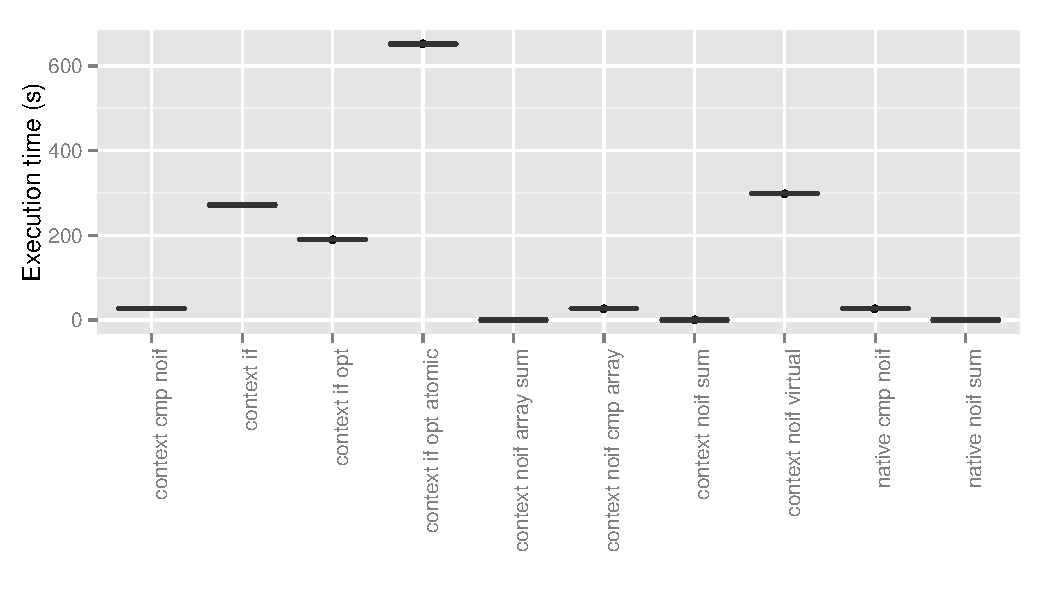
\includegraphics[scale=0.8]{benchmarkif}
\caption[Benchmark of implementation choices.]{Benchmark of implementation choices~\cite{raab2014program}.
The figure shows a boxplot with linear scale.
Because of the large scale, the boxes are only (thick) lines.
\figref{benchmarkcmp} shows the boxes of the three fastest variants.
Black dots indicate measurements not within $1.5*$interquartile range~\cite{raab2015global}}
\label{fig:benchmarkif}
\end{figure}

For the next four microbenchmarks, we compare the performance on the contextual class ^Integer^ instead of the native value of type ^uint32_t^ using the following code~\cite{raab2014program}:

\begin{code}[language=Cpp]
Integer::type add_contextual (Integer const & i1,
				              Integer const & i2)
{
	return i1+i2;
}
\end{code}

To make above source code work, we overload the \emph{type conversation operator}.
The type conversation operator in C++ allows contextual values to be used whenever a type ^uint32_t^ is expected~\cite{raab2014program}:

\begin{code}[language=Cpp]
operator uint32_t () const
{
	/* Implementation of different access strategies
	   for contextual values*/
}
\end{code}


\subsubsection{(Atomic) Branches}

A na\"{i}ve approach to update context changes is by checking a tidy flag on every access of the contextual value~\cite{raab2014program}:

\begin{code}[language=Cpp]
operator uint32_t () const
{
	if (m_context_changed)
	{
		update ();
	}
	return m_cache;
}
\end{code}

This specific implementation requires two additional branches for each call of \linebreak ^add_contextual^ with devastating results:
The loop then takes 271.62 seconds (it is ten times slower, see ``context if'' in Figure~\ref{fig:benchmarkif}).
The run-time is improved to 190.13 seconds (\p{30} faster, see ``context if opt''  in Figure~\ref{fig:benchmarkif}) by giving the compiler hints which ^if^-branch is taken more often~\cite{raab2014program}.
Such improvements, however, do not change the overall outcome, the overhead is still high.
Another major drawback of the solution with branches is that the compiler cannot optimize away arithmetic loops~\cite{raab2014program}.
The use of branches for every access, however, yields benefits:
\begin{itemize}
\item
It makes context changes lazy.
Instead of looking up affected contextual value on every context change, we would only mark them as tidy (^m_context_changed^ from above).
\item
When the contextual value facilitates ^std::atomic<bool>^ instead of ^bool^ for ^m_context_changed^, the contextual values are multi-thread safe.
Unfortunately, atomicity adds extra costs:
The resulting run-time of 651.92 seconds is more than doubled if we use an ^atomic^ type (see ``context if opt atomic''  in Figure~\ref{fig:benchmarkif}).
With clang (version ^3.5-1~exp1^ using option ^-O3^) the run-time is 81.42 seconds both for ^std::atomic<bool>^ and ^volatile bool^.
Nevertheless, the results are still far from desired~\cite{raab2014program}.
\end{itemize}


\subsubsection{Virtual Function Calls}


The next implementation technique we discuss is switching objects at run-time.
The only change needed is to provide a base class and add the C++ ^virtual^ modifier~\cite{raab2014program}:

\begin{code}[language=Cpp]
virtual operator uint32_t () const
{
	return m_cache;
}
\end{code}

Virtual function calls are generally believed to outperform switch statements.
Virtual function tables, a possible implementation technique, received attention of the research community, particularly for super-scalar processors~\cite{driesen1996direct,bacon1996fast,calder1994reducing}.
But, virtual function calls (where it is not known which class be called) make some optimizations (especially inlining) impossible~\cite{driesen1996direct}.
In our case, virtual function calls even perform poorer than an ^if^-branch, leaving us with a run-time of 298.8 seconds (see ``context noif virtual''  in Figure~\ref{fig:benchmarkif}).
Optimizations that avoid the whole loop are impossible, too~\cite{raab2014program}.


\subsubsection{Member Array}

The next method is a member array containing values for every context.
Context changes are represented by modifying the array index ^m_index^, again using the observer pattern.
On access of the contextual value, we return an element of the array~\cite{raab2014program}:

\begin{code}[language=Cpp]
operator uint32_t () const
{
	return g_arr[m_index];
}
\end{code}

Such member arrays yield promising results:
27.16 seconds (see ``context noif cmp array''  in Figure~\ref{fig:benchmarkif} and later in \ref{fig:benchmarkcmp}).
Additionally, optimizations can completely eliminate arithmetic loops~\cite{raab2014program}.%
{\parfillskip=0pt plus .8\textwidth \emergencystretch=.5\textwidth \par}

An array with elements for every combination of activated layers has a drawback:
Done in a na\"{i}ve way it needs a large amount of memory for each contextual value because the number of layer combinations easily gets huge.
We left optimizations of this technique as a future work~\cite{raab2014program}.

\subsubsection{Member Variable}

The most efficient implementation is the use of one memory cell per contextual value and returning its content directly~\cite{raab2014program}:

\begin{code}[language=Cpp]
operator uint32_t () const
{
	return m_cache;
}
\end{code}

With this technique we measured a median of 27.16 seconds (see ``context cmp noif'' in figures~\ref{fig:benchmarkif} and \ref{fig:benchmarkcmp}).
We got the same result as with the native variable access (``native cmp noif''), which means that we did not measure any overhead.
Furthermore, the technique requires only minimal memory for caching (one native type per contextual value).
Of course, we must look up values on layer activation~\cite{raab2014program}.

\subsubsection{Discussion}

It is not surprising that such a simple variable access performs well.
Nevertheless, we cannot claim that the optimizations (we rely on) are done by every compiler for every program.
We answer our research question:
\rqFrontendTradeOff*

\begin{finding}
Both member arrays and member variables have no overhead in our benchmark.
The use of member variables has minimal space requirements.
\end{finding}

We decided to use the member variable implementation technique because it had no run-time overhead in the benchmark on read-only access.
Furthermore, the technique has minimal memory overhead, fulfilling our requirement:
\reqFast*

We will elaborate on this benchmark, and evaluate the costs of layer activations much later in \secref{evaluation-context-aware}.
















\section{Multi-threaded Contextual Values}
\label{sec:seus}

In this section we extend \elektra{} to ubiquitous computing.
We found a combination of three problems in this domain:

\begin{description}
\item[Context awareness]
aims to impress users by letting devices react in smart ways.
Devices shall consider properties of their physical environment and information users gave them.
For example, if a smart phone is taken out of the pocket, the phone does not measure body temperature anymore.
In this situation, the phone turns off vibration because the user would not feel it anyway~\cite{raab2015global}.
\item [Customizability]
aims to give end users the opportunity to modify unwanted default values and context awareness, hence bringing the behavior in line with their needs.
For example, if users are deaf, turning off vibration is not a good solution~\cite{raab2015global}.
\item [Performance on multi-core processors]
bear new challenges and are accepted as an upcoming trend for embedded computing.
Multi-threading is an attractive technique to more thoroughly facilitate multi-core processor resources~\cite{raab2015global}.
\end{description}

In the previous section we mainly addressed context awareness and customizability.
In this section we extend \elektra{Lib} with support for multi-threading.
We aim at context activations across threads.
For example, if context sensors detect that the battery is low, we want to have a mechanism that notifies all threads of each running application~\cite{raab2015global}.

\subsection{Introduction of Embedded Use Case}

We describe an embedded use case as often found in ubiquitous computing.
Let us consider a ubiquitous computing device that shall be protected via a watchdog:

\begin{code}
[watchdog/%security%/enabled]
  type:=boolean
  default:=1
\end{code}

In the example above, we specify ^enabled^ as contextual value.
We use ^boolean^ as its type.
\elektra{Gen} generates the source code implementing the contextual values.
\elektra{Gen} reads the specification above and emits the classes ^Environment^, ^Watchdog^, and ^Enabled^~\cite{raab2015global}.

A single contextual value has a countable, infinite number of values: one value for every relevant context.
These values are available in a key set.
The unique key name required to look up individual values is resolved by substitution of the context placeholders~\cite{raab2015global}.

\begin{code}[language=Cpp]
void printWatchdogStatus (Watchdog::Enabled const & e)
{
	if (e) { cout << "Watchdog is enabled"; }
}
\end{code}

In \elektra{}, contextual values are only subject to be changed iff at least one of the context placeholders in the specification coincides with the layer name~\cite{raab2015global}:

\begin{code}[language=Cpp]
void enableWatchdogInHighSecurity (Watchdog::Enabled & e)
{
	bool originallyEnabled = e;
	assert (e.getName () == "/watchdog/%/enabled");
	e.context ().with<Security> ("high")([&]{
		e = true; // security context "high" active here
		assert (e.getName () == "/watchdog/high/enabled");
	}); // end of security context "high"
	assert (e == originallyEnabled);
	assert (e.getName () == "/watchdog/%/enabled");
}
\end{code}

In line~3, we see a read-access of the contextual value ^e^.
In line~4, we assert that no ^security^ context was set before, by checking that the context placeholder ^%security%^ is replaced by a ^%^, i.\,e., an empty layer.
In line~5, we activate the layer ^Security^ with the argument ^"high"^ for the layer construction.
The lambda function (block after the capture list \lstinline[language=Cpp]^[&]^) is executed in the same thread but in another context.
In line~9, the contextual value ^e^ again has the value and context as before because we left the block where ^Security^ was activated.
The function has a side effect:
The contextual value ^e^ is modified in the security-context ^high^.
After calling this function and serializing the configuration settings, we get the resulting configuration setting~\cite{raab2015global}:

\begin{code}[language=CfgElektra]
watchdog/high/enabled=1
\end{code}

\subsection{Synchronization Points}


In its essence, our extension defines \intro[synchronization point]{synchronization points} for multi-thread-safe synchronization of layers and contextual values.
At these synchronization points global locks ensure sequential activations and deactivations.
We leave priority concerns to threading facilities of the operating system~\cite{raab2015global}.
We implement our extension as ^ContextPolicy^ (see \secref{approach-policy}) called ^ThreadContext^.

Because programs access contextual values frequently but change context less frequently, \elektra{} avoids overhead while reading the value.
We achieve this behavior by demanding the introduction of synchronization points by the developer.
Code executed at the synchronization points pushes new values to contextual values using the observer pattern.
We gain two advantages:
\begin{itemize}
\item
Performance overhead occurs exclusively during synchronization points and assignments.
Reading contextual values still has the same overhead as accessing native variables~\cite{raab2014program}.
\item
Another advantage of synchronization points is that the user has full control over resource consumption including battery drain that is important for most battery-powered devices~\cite{raab2016persistent}.
\end{itemize}

The first synchronization point we introduce is ^syncLayers^.
The thread of execution uses ^syncLayers^ to have identical active layers to that it would have had if it had executed every ^activate^ and ^deactivate^ of the program itself.
After every thread has called ^syncLayers^, the whole process has the same active layers.

\begin{example}
Let us consider two threads with a ^ThreadContext^ ^c1^ and ^c2^, respectively:

\begin{multicols}{2}
\begin{code}[language=Cpp,xleftmargin=0ex,xrightmargin=0ex]
c1.activate<BatteryLow> ();

\end{code}

\columnbreak

\begin{code}[language=Cpp,xleftmargin=0ex,xrightmargin=0ex,numbers=right]

c2.syncLayers ();
\end{code}
\end{multicols}

The ^Context^'s method ^syncLayers^ updates the layers of the context ^c2^ accounting for the ^activate^ in ^c1^, which happened before.
After execution of ^c2.syncLayers^, the layers in ^c2^ are at par to the context of the other thread ^c1^.
\end{example}


The need of placing synchronization points seems to be cumbersome when programming.
In practice, however, these places are usually evident---when users start new interactions.
With a use-case-based approach to software engineering developers systematically find all such places.
For optimization purposes, users can avoid synchronization points at less important places.
Global optimizations are possible, too.
For example, we can ignore synchronization points if we visited one a short time ago.
In some architectures we completely remove synchronization points from the main concerns.
For example, in architectures with short interactions and notifications on context changes~\cite{raab2016persistent}.
In some situations this explicit definition of checkpoints yields an advantage.
For example, if an algorithm assumes variables to be constant.
Then the developer has a way to specify where updates are done safely~\cite{raab2015global}.

\begin{example}
Consider an algorithm that must terminate sooner if the battery is low.
Because of the reduction of computation, the device would consume less power.
As a first step, we specify a contextual value that defines the accuracy for this algorithm~\cite{raab2015global}:

\begin{code}
[algorithm/%batterylow%/accuracy]
  type:=long
  default:=100
\end{code}

As second step, we add a synchronization point before the algorithm.
Afterwards, the algorithm calculates its task without any overhead~\cite{raab2015global}:

\begin{code}[language=Cpp]
void userInteraction (Algorithm::Accuracy const & accuracy)
{
	accuracy.context ().syncLayers (); // sync accuracy
	for (long i=0; i<accuracy; ++i)
	{
		// calculate Task with given accuracy
		// contextual value is not changed within loop
	}
}
\end{code}

The method ^context^ returns the ^ThreadContext^ associated with the contextual value ^accuracy^.
Then we define a synchronization point using its method ^syncLayers^.
Every time a synchronization point is passed, all layer changes in other threads are taken into account~\cite{raab2015global}.
The developer is certain that ^accuracy^ is not changed during the loop starting on line~4 at unwanted places~\cite{raab2016persistent}.
\end{example}


\subsection{Global Activation}

We extend our frontend so that ^activate^ and ^deactivate^ work across threads~\cite{raab2015global}.
Let us specify a contextual value that provides a security level based on the tampering of the device:

\begin{code}
[security/%tampered%/level]
  type:=long
  default:=high
\end{code}

Then we share the contextual value in a multi-threaded program with two threads.
The local variables ^c1^ and ^c2^ represent the context in the respective left and right thread.
They keep track of the currently active layers of their own threads:

\begin{multicols}{2}
\begin{code}[language=Cpp,xleftmargin=0ex,xrightmargin=0ex]
c1.deactivate<Tampered> ();

// Security unchanged
// (missed update)
\end{code}

\columnbreak

\begin{code}[language=Cpp,xleftmargin=0ex,xrightmargin=0ex,numbers=right]
Security.Level sl (ks, c2);

c2.activate<Security> (sl);
// Tampered now deactivated
\end{code}
\end{multicols}

After \empha[synchronization point]{synchronization points}, contexts integrate layer switches that occurred in other threads.
Every ^activate^ and ^deactivate^ works as synchronization point.
On the left thread in line~1, we deactivate the layer ^Tampered^.
The change happens immediately in the left thread but needs till line~3 of the right thread because no synchronization point occurs earlier.
The activation in line~3 pulls the deactivated layer to the context ^c2^.
Thus the contextual value ^sl^ (security level) is affected by the layer change of ^Tampered^.
\elektra{} guarantees that ^sl^ gets aware of its new context before the ^Security^ layer gets activated.
At the end of the left side's thread, the layer ^Tampered^ is deactivated and ^Security^ has the value it had in ^c1^ from the beginning.
At the end of the right side's thread, ^Tampered^ is deactivated and ^Security^ is activated.
All contextual values connected with ^c2^, including ^sl^, are updated at that point.

We implicitly synchronize all layers with any activation to be sure that the activation is not using out-dated information.
The synchronization of layers before layer (de)activations itself is a preferable property:
This way we guarantee that every context in every thread consists of the same activated layers with the same layer values.
This is essential if we activate a layer that internally uses contextual values.
Without layer synchronization done first, the contextual values used during activations would have wrong values.
We want to avoid that because of our requirement:
\reqConsistency*

\subsection{Coordination}
\label{sec:thread-context}

\begin{figure}[htp]
\centering
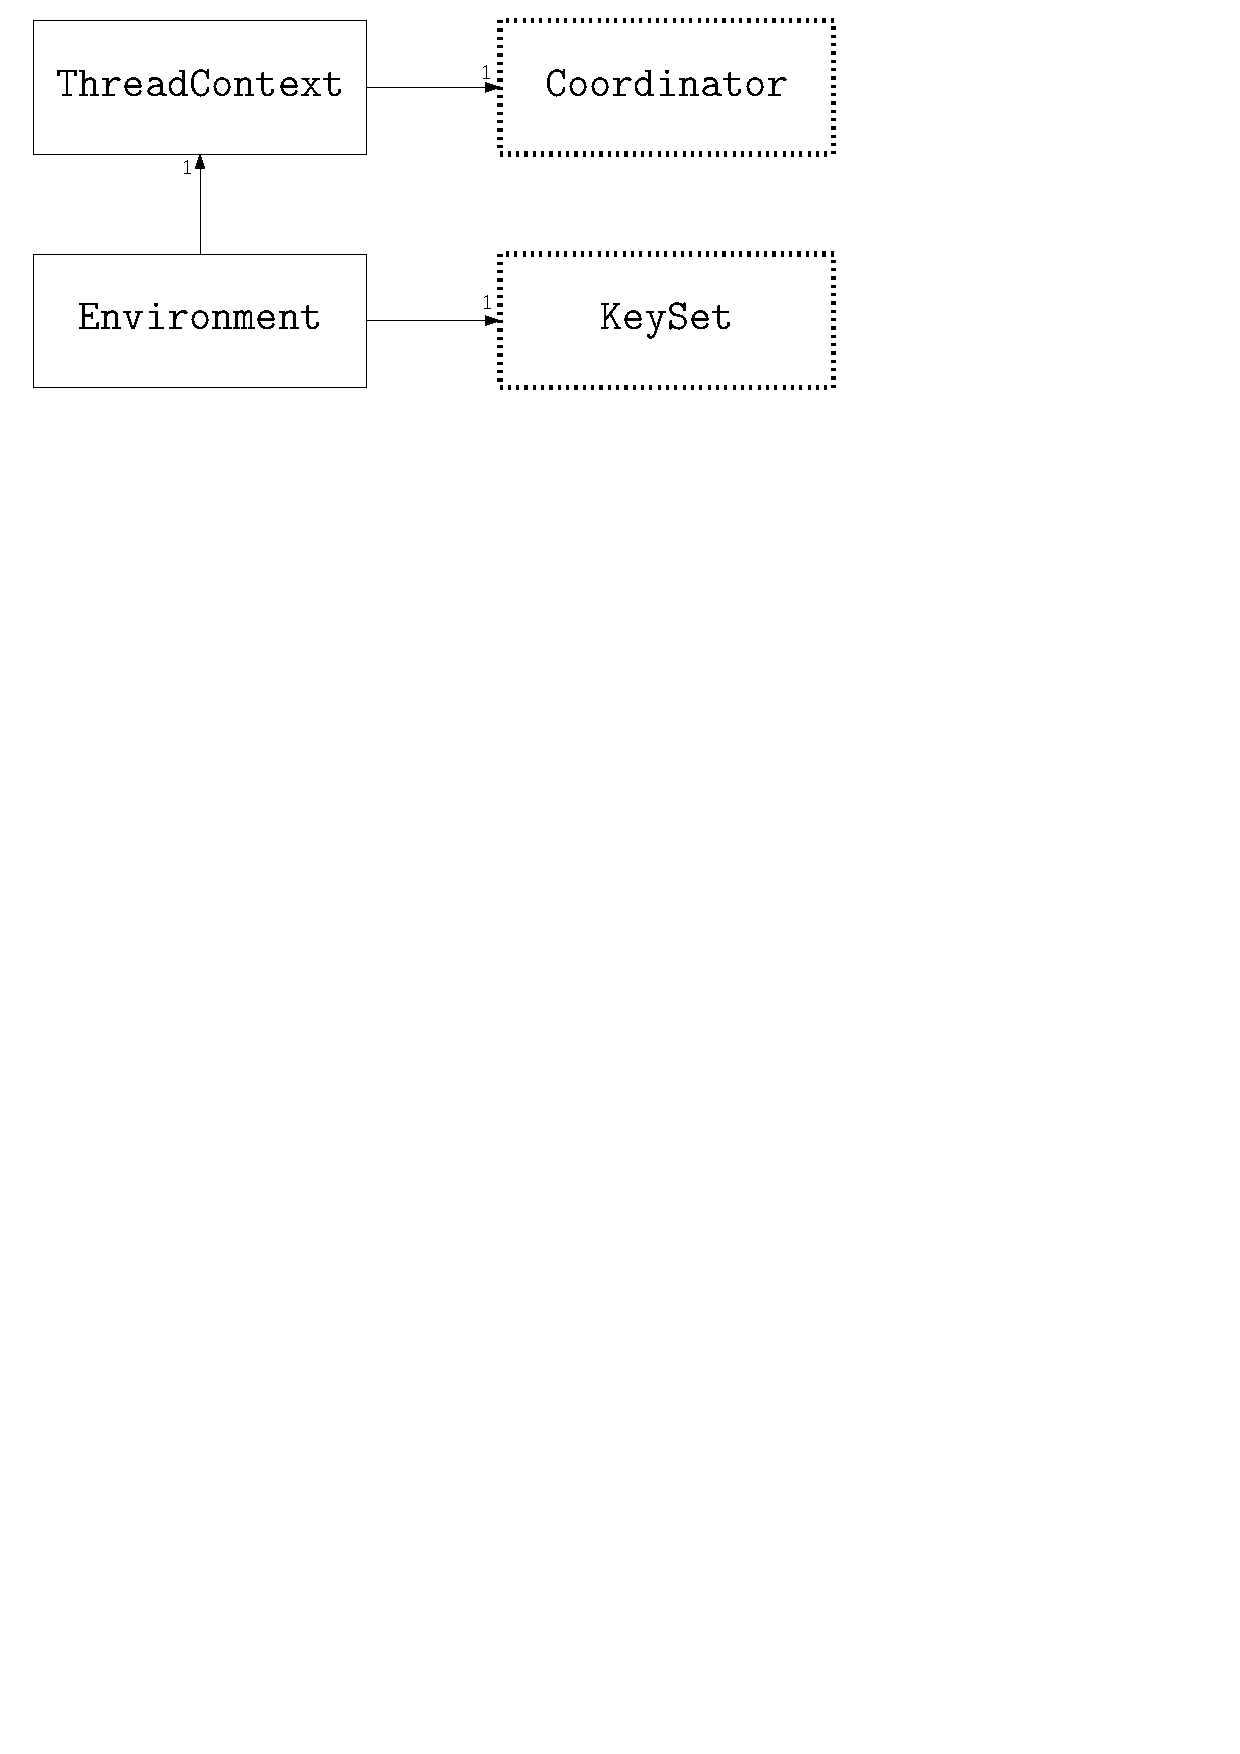
\includegraphics[scale=0.6]{coordination}
\caption[Coordination between threads.]{Coordination between threads, showing the major components involved. The dotted boxes are to be shared between threads. Arrows express a composition~\cite{raab2015global}.}
\label{fig:coordination}
\end{figure}

In Figure~\ref{fig:coordination} we display the major parts necessary for coordination between contextual values.
The key set is used as the set of all values in every context as needed for lookup and serialization.
The class ^Environment^ is the generated class hierarchy's root.
Objects of ^ThreadContext^ encapsulate all layers active in one thread.
As the name suggests, every thread uses its own ^ThreadContext^.
Finally, the ^Coordinator^ guards coordination between ^ThreadContext^.
The boxes, which are drawn with the dotted dash style, are only instantiated once per process and are shared between all threads~\cite{raab2015global}.

We do not need any locks or atomic values in ^KeySet^, ^ThreadContext^ nor the ^Environment^ (the contextual values).
Instead we delegate all coordination work to objects of the class ^Coordinator^.
Both ^ThreadContext^ and ^Coordinator^ employ the observer pattern internally.
By the use of callbacks, we completely decouple the coordination and the key sets~\cite{raab2015global}.

Applications do not have restrictions of how many objects of the class ^Coordinator^ or ^KeySet^ are used.
They can be used within plugins or otherwise nested applications.
Nevertheless, \elektra{} imposes the following constraints:
Every ^Coordinator^ is bound to exactly one ^KeySet^, every ^ThreadContext^ is liable to exactly one ^Coordinator^, and again every contextual value is accountable for exactly one ^ThreadContext^~\cite{raab2015global}.

\subsubsection{Assignment}

Suppose ^value^ is specified to be a contextual value of type long integer~\cite{raab2015global}:

\begin{code}
[value]
  type:=long
  default:=0
\end{code}

Then we assign and use the contextual value as an integer in source code~\cite{raab2015global}:

\begin{code}[language=Cpp]
value = 8;
assert (value == 8);
\end{code}

Different from reading contextual values, the assignment of contextual values has additional overhead.
For every change of the value, next to the cache, the underlying key set needs to be updated in a thread-safe way.
The design decision is because of the assumption that customization (assignment) occurs less often than accessing values and changing layers.
The decision leads to desired properties:
\begin{enumerate}
\item 
Freshly created contextual values have an up-to-date value with respect to assignments, even across threads~\cite{raab2015global}:
\begin{multicols}{2}
\begin{code}[language=Cpp,xleftmargin=0ex,xrightmargin=0ex]
value = 5;



\end{code}

\columnbreak

\begin{code}[language=Cpp,xleftmargin=0ex,xrightmargin=0ex,numbers=right]

ThreadContext tc (c);
Value value (ks, tc);
assert (value == 5);
\end{code}
\end{multicols}

\item
The data structure key set is kept up to date and its serialization always contains the latest assignments~\cite{raab2015global}.
\end{enumerate}





\subsubsection{Thread-based Layers}
\label{sec:thread-layer}


Layers, that compare the current thread identification with a selected thread identification, are a powerful technique.
When these layers are activated globally, they selectively influence threads~\cite{raab2015global}.

\begin{example}
We want to activate a layer only within a single thread specified with the thread identification ^m_selected^.
Implementing this layer is straightforward~\cite{raab2015global}:

\begin{code}[language=Cpp]
class Thread : public Layer
{
public:
	Thread (pthread_t selected) :
		m_selected (selected) {}
	string id () const { return "thread"; }
	string operator() () const {
		if (pthread_self () == m_selected) return "active";
		return "";
	};
private:
	pthread_t m_selected;
};
\end{code}

At line~8, we have to check if the current thread identification is identical to the thread identification of a selected thread.
The method ^pthread_self^ tells us the thread identification of the calling thread.
If the current thread is the selected thread, we return that the layer is ^"active"^.
Otherwise, we return an empty string to tell that the layer is deactivated~\cite{raab2015global}.
\end{example}


The same technique is applied to change the context for a pool of threads.
Instead remembering a single selected thread, we remember a set of relevant threads~\cite{raab2015global}.





\subsection{Result and Use}

Here we answer the research question:
\rqFrontendConcurrent*

\begin{finding}
We improve contextual values by defining synchronization points that allow thread-safe use of contextual values and layer activations across selected threads.
\end{finding}

We described an extension in which we use the policy implementation ^ThreadContext^ instead of ^Context^ (from the previous \secref{cop}).
For multi-threaded applications, we have to set ^ContextPolicyIs^~\cite{raab2015global} (see \secref{approach-policy} for details of ^ContextPolicy^).

A function ^main^ that uses multi-threaded \elektra{} can be written as follows~\cite{raab2015global}:

\begin{code}[language=Cpp]
int main (int argc, char ** argv)
{
	KeySet ks;
	ksGetOpt (argc, argv, ks);
	KDB kdb;
	kdb.get (ks);
	Coordinator c;
	ThreadContext tc (c);
	Environment<ContextPolicyIs<ThreadContext>> env (ks,tc);
	// the rest of the program using env
}
\end{code}


The ^ContextPolicyIs^ in line~9 changes the policy class for all contextual values for this instantiation of the ^Environment^.





\section{Persistent Contextual Values as Inter-process Layers}
\label{sec:mobile}

While the manually written layers provide some opportunities as shown in \secref{thread-layer}, in nearly all cases the layers are boilerplate code pursuing the same goals:
\begin{enumerate}
\item Making activation of layers \emph{context aware}:
Here we need to take a contextual value as parameter for the layer.
\item Allowing \emph{persistence} of layers:
Doing so, we share layers across applications.
\end{enumerate}

In this section we describe the novel idea to use contextual values for layer activation, avoiding manual implementation of layers.
We aim at combining layer activations with contextual values fulfilling the goals above.
We suggest to use contextual values as parameters to ^activate^ and ^with^.
Because contextual values are context aware, by definition, they always consider their context.
By persisting contextual values we enable synchronization of layer activations between applications.
We keep our previous performance properties:
Reading contextual values is as fast as reading native variables~\cite{raab2016persistent}.

\begin{example}
Let us consider internationalized software.
As a prerequisite, we need a specification shared between applications:

\begin{code}
[language]
  type:=string
  default:=english
[person/%language%/greeting]
  type:=string
  default:=hello
\end{code}

Using this specification a code generator yields the classes ^Person^, ^Greeting^, and ^Language^.
The classes ensure contextual value semantics.

Contextual values help us, for example, to easily display translated messages.
Using the concepts as introduced before, it is difficult to ensure that every application has activated the same language.
We would need to activate the correct layer in every application individually.
There was no straightforward way for one application to tell all other applications that the language has changed.
We propose to activate such layers with code-generated contextual classes (such as ^Language^)~\cite{raab2016persistent}:

\begin{code}[language=Cpp]
void greet (Person const & p, Language const & language)
{
	p.activate (language);
	cout << p.greeting << endl;
}
\end{code}

In line~3 we activate the contextual value ^language^.
The execution environment initializes contextual values at application startup, providing sensible default values changeable by settings for different contexts.
The build-in persistence of key sets allows us to activate the same layer across applications~\cite{raab2016persistent}.
\end{example}

The rest of the section is structured as follows:

\secref{frontend-inter-process-layers}: We describe the semantics of inter-process layers.

\secref{frontend-intra-process-notification}: An intra-process notification system is allowing us to update the context of contextual values when other contextual values, representing layers, change.

\secref{frontend-inter-process-notification}: An inter-process notification system is telling us when to reparse configuration files.


\subsection{Inter-process Layers}
\label{sec:frontend-inter-process-layers}

Because we use contextual values as layers, all properties of context specifications are reused.
The only missing information to enable activation of contextual values is the layer name.
To make specifications more compact, we decided that by default the layer name is the basename of the contextual key names.
This convention yields appropriate layer names for most contextual values~\cite{raab2016persistent}.

\begin{example}
Let us define a contextual value to be used as layer:

\begin{code}
[%language%/country]
  default:=
\end{code}

The contextual value ^country^ has the layer name ^country^.
\end{example}

Layer names, unlike contextual values, do not form a hierarchy.
In some situations the basename does not present the right choice.
In such situations we use the property value of~\property{layer/name} to select a layer name.

\begin{example}
Let us facilitate a country code to identify countries~\cite{raab2016persistent}:

\begin{code}[morekeywords={name}]
[country/%language%/code]
  type:=string
  layer/name:=country
  default:=C
\end{code}

Because the layer name ^code^ (derived from the basename) would be too generic, we use property~\property{layer/name} to rename it.
Then activating the contextual value ^env.^\allowbreak^country.code^ activates the layer ^country^~\cite{raab2016persistent}.
\end{example}

We have a complete context specification as necessary for contextual values and layers, fulfilling the requirement:
\reqSpecification*

\subsubsection{Context-aware Activation}

With this extension, developers do not have to consider context when activating layers.
Context-aware activations correctly consider up-to-date contextual values.

\begin{example}
Let us define some contextual values~\cite{raab2016persistent}:

\begin{code}
[location]
  type:=string
  description:=GPS position in ??N??W
  default:=
[%location%/country]
  type:=string
  default:=
[person/%country%/greeting]
  type:=string
  default:=Hello
\end{code}

To activate the layer ^country^ and ^location^ we use~\cite{raab2016persistent}:

\begin{code}[language=Cpp]
void greet (Person & p, Country & country, Location & location)
{
	p.context ().activate (location);
	p.context ().activate (country);
	cout << p.greeting << endl;
}
\end{code}

If ^location^ and ^country^ would be layers without contextual values as described in earlier sections, exactly these layers would be activated without influencing each other.
This means that ^activate^ in line~4 would not take the location changed in line~3 into account.
But since ^location^ and ^country^ are contextual values (implemented by the contextual classes ^Location^ and ^Country^), they factor in context and the activations correctly influence each other.
In the example above, after the activation of the contextual value ^location^, the position of the contextual value  ^country^ is updated.
Line~4 updates the contextual value ^country^ as needed by the established context~\cite{raab2016persistent}.
Given the configuration settings:

\begin{code}[language=CfgElektra]
location=48N16O
48N16O/country=austria
person/austria/greeting=Griaz enk!
\end{code}

The output of the program is:

\begin{code}
Griaz enk!
\end{code}
\phantom{}
\end{example}

\subsubsection{Activation via Assignment}

A not-so-obvious property of activating contextual values is that, after activation, developers control (^de^)^activation^ via changing the values of contextual values~\cite{raab2016persistent}.

\begin{example}
We deactivate the layer location by an assignment:

\begin{code}[language=Cpp]
void emptyGreet (Person & p, Location & location)
{
	location = "";
	p.activate (location);
	cout << p.greeting << endl;
}
\end{code}

After line~3, the contextual value ^location^ has an empty string in its current context.
In line~4 we activate the layer ^location^.
Despite the activation, because of the empty value, the context placeholder ^location^ is replaced with ^%^, i.\,e., it is deactivated.
The greeting in line~5 is according to a deactivated layer location.
\end{example}


\begin{example}
No layer switch occurs after we have done a deactivation of a contextual value:

\begin{code}[language=Cpp]
void assignLanguage (Language & language)
{
	language.context ().activate (language);
	language = "";
	// layer language deactivated
	language = "spanish";
	// layer switch to spanish
	language.context ().deactivate (language);
	language = "english";
	// layer still deactivated
}
\end{code}

As precondition, to make contextual values act as a layer, we activate the contextual value (line~3).
Layers with an empty value (line~4) impact contextual values in the same way as otherwise deactivated layers:
Placeholders are replaced with ^%^.
Only after explicit deactivation in line~8, assignments of the contextual value ^language^ do not interfere with other contextual values anymore~\cite{raab2016persistent}.
\end{example}

In summary we have two different ways to deactivate layers:
\begin{enumerate}
\item We call ^deactivate^ with the contextual value as parameter.
\item We activate a contextual value that contains an empty string or assign an empty value to an already activated contextual value.
\end{enumerate}

The different deactivations have an important difference:
A layer with an empty value can be activated by assigning a different string, which is not possible after calling ^deactivate^.



\subsection{Intra-process Notification}
\label{sec:frontend-intra-process-notification}

In previous sections we assumed that changes of a contextual value only happen by an assignment to a contextual value.
In this extension we do not need this assumption anymore.
We introduce a reloading mechanism for updates of the underlying key set~\cite{raab2016persistent}.

For such in-memory synchronizations we provide the method ^sync^~\cite{raab2016persistent}.
Invoking ^sync^ updates all contextual values with the values the key set currently has and makes sure that correct layers are active afterwards.

\begin{example}
\label{ex:do-sync}
To fetch the latest configuration settings from the hard disk and update all contextual values according to the new configuration settings, we use:

\begin{code}[language=Cpp]
void doSync (Context & c, KDB & kdb, KeySet & ks)
{
	kdb.get (ks);
	c.sync ();
	// contextual values are updated;
	// and layers are activated accordingly
}
\end{code}

In line 3 we update the ^KeySet ks^, which is connected with the contextual values.
In line 4 we execute the in-memory update to reload the contextual values~\cite{raab2016persistent}.
\end{example}

The behavior of the synchronization via ^sync^ does not differ from performing ^activate^ or ^deactivate^ via assignment.
Developers can think of ^sync^ as assigning all changed contextual values in the correct order~\cite{raab2016persistent}.

\subsubsection{Activation Order}

For correct behavior of ^sync^ we need to consider the dependences between contextual values.
Contextual values with context placeholders (^%...%^) depend on contextual values with a basename identical to the context placeholder's name.
We use a topological sort based on Kahn to order according to the dependences~\cite{kahn1962topological,raab2016persistent}.

As long as layers and contextual values were completely separate concepts, we cannot build dependence cycles:
It was not possible that layers depend on contextual values.
Activation of contextual values, however, introduces the possibility of cyclic dependences.

\begin{example}
We need at least two contextual values to build a cycle~\cite{raab2016persistent}:


\begin{code}
[%country%/language]
  type:=string
  default:=
[%language%/country]
  type:=string
  default:=
\end{code}

Then we need to craft configuration settings to make use of the cycle:

\begin{code}[language=CfgElektra]
swiss/language=de
luxembourg/language=fr
fr/country=swiss
de/country=luxembourg
\end{code}

If the application activates the layer ^country^, \elektra{} would need the value of the ^language^ layer and vice versa.
Activation of layers within such cycles lead to toggling values~\cite{raab2016persistent}.%
{\parfillskip=0pt plus .8\textwidth \emergencystretch=.5\textwidth \par}
\end{example}

Luckily such cycles only stem from design errors and are unwanted.
Thus we prohibit such cycles already in the context specification.
These situations shall be detected early by checking the specification~\cite{raab2016persistent}, following the requirement:
\reqGeneration*




\subsection{Inter-process Notification}
\label{sec:frontend-inter-process-notification}

Because of diverse requirements in different applications and systems, we took care that \elektra{} exhibits  modular design principles~\cite{raab2010thesis,raab2016improving}.
We decided to give applications different inter-process notification methods to choose from~\cite{raab2016persistent}, complying with the Requirement~\reqref{legacy}:
\reqLegacy*


Whenever processes use ^kdb.set^ to modify the underlying configuration files the notification mechanisms fire.
Every interested process listens to the notifications and then fetches the updated configuration settings using ^kdb.get^.
Once every thread has passed a synchronization point, the application is fully up to date~\cite{raab2016persistent}, fulfilling the requirement:
\reqConsistency*


\label{sec:three-way-merge}
As shown in \exref{do-sync}, ^kdb.get^ updates the contextual values.
On conflicts \elektra{} supports a three-way merge~\cite{raab2016persistent}.
A \intro{three-way merge} implies that we consider the common ancestor next to our internal (the application's) and the external (the system's) configuration settings.
Using a three-way merge, we avoid errors in situations where configuration settings are clearly changed by one party (either internal or external).
If both sides change the same configuration value conflictingly, the three-way merge cannot help and we usually need to propagate the decision to the user.

With inter-process notification in place, we answer the research question:
\rqFrontendUsability*

\begin{finding}
We found that most of the time, contextual values have the necessary information to be used as replacement to manual implementation of layers.
As main benefit, we always get context-aware layer activation.
Using persistence and inter-process notification, we share layer information between applications.
\end{finding}



